\documentclass[coursework]{SCWorks}

\usepackage{preamble}

\begin{document}

\chair{математической кибернетики и компьютерных наук}

\title{Алгоритмы сортировки}

\course{1}

\group{111}

\napravlenie{02.03.02 "--- Фундаментальная информатика и информационные технологии}

\author{Лебедева Семёна Юрьевича}

\chtitle{доцент, к.\,ф.-м.\,н.}
\chname{С.\,В.\,Миронов}

\satitle{доцент, к.\,ф.-м.\,н.}
\saname{Г.\,Г.\,Наркайтис}

\patitle{доцент, к.\,ф.-м.\,н.}
\paname{С.\,В.\,Миронов}

\nirtitle{доцент, к.\,п.\,н.}
\nirname{В.\,А.\,Векслер}

\term{2}
\practtype{учебная}
\duration{2}
\practStart{01.09.2025}
\practFinish{30.12.2029}

\date{2026}

\maketitle

\secNumbering

\tableofcontents

\intro

Сортировка~--- одна из фундаментальных задач информатики.
Под сортировкой понимается процесс упорядочивания элементов некоторого
множества по заданному критерию~\cite{Knuth}. Эффективные алгоритмы
сортировки лежат в основе баз данных, поисковых систем и многих других
приложений.

В данной курсовой работе рассматриваются три классических алгоритма
сортировки: пузырьковая сортировка, сортировка слиянием и быстрая
сортировка. Для каждого алгоритма приводится теоретический анализ
временной сложности, реализация на языке \texttt{C++}, а также
экспериментальное сравнение производительности.

\section{Теоретические основы алгоритмов сортировки}

\subsection{Пузырьковая сортировка}

Пузырьковая сортировка~--- простейший алгоритм, который последовательно
сравнивает соседние элементы и меняет их местами, если они стоят в
неправильном порядке~\cite{Knuth}. Несмотря на свою простоту, алгоритм
обладает плохой временной сложностью и практически не применяется в
промышленных системах.

Количество сравнений в худшем случае для массива из \(n\) элементов:

\begin{equation}
    \label{eq:bubble}
    C_{\text{bubble}}(n) = \sum_{i=1}^{n-1} i = \frac{n(n-1)}{2} = O(n^2).
\end{equation}

\subsection{Сортировка слиянием}

Сортировка слиянием~--- алгоритм типа «разделяй и властвуй»
(\textit{divide and conquer})~\cite{Cormen}. Массив рекурсивно
разбивается на две половины, каждая сортируется отдельно, затем
отсортированные половины сливаются в один массив.

Рекуррентное соотношение для числа операций:

\begin{equation}
    \label{eq:mergesort}
    T(n) = 2T\!\left(\frac{n}{2}\right) + \Theta(n),
\end{equation}

решением которого по теореме Мастера является \(T(n) = \Theta(n \log n)\).

\subsection{Быстрая сортировка}

Быстрая сортировка (\textit{quicksort}) также относится к классу
«разделяй и властвуй». Выбирается опорный элемент (\textit{pivot}),
массив разбивается на два подмассива~--- меньше и больше опорного~---
и каждый сортируется рекурсивно~\cite{Hoare}.

Ожидаемое число сравнений при случайном выборе опорного элемента:

\begin{equation}
    \label{eq:quicksort}
    E[C(n)] = 2n \ln n - \frac{2(n-1)}{n} \approx 1{,}386\, n \log_2 n.
\end{equation}

\subsection{Сравнительная таблица}

В таблице~\ref{tab:complexity} приведено сравнение временной и
пространственной сложности рассматриваемых алгоритмов.

\begin{table}[H]
    \centering
    \caption{Сравнение сложности алгоритмов сортировки}
    \label{tab:complexity}
    \begin{tabular}{|l|c|c|c|c|}
        \hline
        \textbf{Алгоритм} &
        \textbf{Лучший случай} &
        \textbf{Средний случай} &
        \textbf{Худший случай} &
        \textbf{Память} \\
        \hline
        Пузырьковая & $O(n)$        & $O(n^2)$      & $O(n^2)$      & $O(1)$        \\
        \hline
        Слияние     & $O(n \log n)$ & $O(n \log n)$ & $O(n \log n)$ & $O(n)$        \\
        \hline
        Быстрая     & $O(n \log n)$ & $O(n \log n)$ & $O(n^2)$      & $O(\log n)$   \\
        \hline
    \end{tabular}
\end{table}

\section{Реализация алгоритмов}

Все алгоритмы реализованы на языке \texttt{C++17}~\cite{Stroustrup}
в виде шаблонных функций в файле \texttt{sorting.cpp}
(см.~приложение~\ref{app:fullcode}). Использование шаблонов позволяет
сортировать любые типы данных, для которых определён оператор
\mintinline{cpp}{operator<}.

\subsection{Пузырьковая сортировка}

Функция \mintinline{cpp}{bubbleSort} принимает итераторы начала и
конца диапазона, аналогично функциям стандартной библиотеки. Флаг
\mintinline{cpp}{swapped} позволяет прервать цикл досрочно, если за
текущий проход не было ни одного обмена~--- это даёт сложность $O(n)$
на уже упорядоченных данных (см.~формулу~\ref{eq:bubble}).

\begin{minted}{cpp}
template <typename It>
void bubbleSort(It first, It last) {
    for (auto i = first; i != last; ++i) {
        bool swapped = false;
        for (auto j = first; j != std::prev(last, i - first + 1); ++j) {
            if (*std::next(j) < *j) {
                std::iter_swap(j, std::next(j));
                swapped = true;
            }
        }
        if (!swapped) break;
    }
}
\end{minted}

\subsection{Сортировка слиянием}

Функция \mintinline{cpp}{mergeSort} рекурсивно делит диапазон пополам
и вызывает вспомогательную функцию \mintinline{cpp}{merge} для слияния
двух упорядоченных половин. Временная буферная память выделяется
однократно и передаётся через параметр \mintinline{cpp}{buf}.

\begin{minted}{cpp}
template <typename It>
void merge(It first, It mid, It last, std::vector<typename It::value_type>& buf) {
    buf.clear();
    auto l = first, r = mid;
    while (l != mid && r != last)
        buf.push_back(*l < *r ? *l++ : *r++);
    buf.insert(buf.end(), l, mid);
    buf.insert(buf.end(), r, last);
    std::copy(buf.begin(), buf.end(), first);
}

template <typename It>
void mergeSort(It first, It last, std::vector<typename It::value_type>& buf) {
    if (std::distance(first, last) <= 1) return;
    auto mid = std::next(first, std::distance(first, last) / 2);
    mergeSort(first, mid, buf);
    mergeSort(mid, last, buf);
    merge(first, mid, last, buf);
}
\end{minted}

\subsection{Быстрая сортировка}

Функция \mintinline{cpp}{quickSort} использует в качестве опорного
элемента медиану из первого, среднего и последнего элементов
подмассива~--- это снижает вероятность вырожденного случая $O(n^2)$
(см.~формулу~\ref{eq:quicksort}).

\begin{minted}{cpp}
template <typename It>
It medianOfThree(It first, It last) {
    auto mid = std::next(first, std::distance(first, last) / 2);
    --last;
    if (*mid < *first) std::iter_swap(first, mid);
    if (*last < *first) std::iter_swap(first, last);
    if (*mid < *last)  std::iter_swap(mid, last);
    return last; // pivot at last
}

template <typename It>
void quickSort(It first, It last) {
    if (std::distance(first, last) <= 1) return;
    auto pivot = medianOfThree(first, last);
    auto p = std::partition(first, std::prev(last),
                            [&pivot](const auto& x){ return x < *pivot; });
    std::iter_swap(p, pivot);
    quickSort(first, p);
    quickSort(std::next(p), last);
}
\end{minted}

\begin{figure}[H]
    \centering
    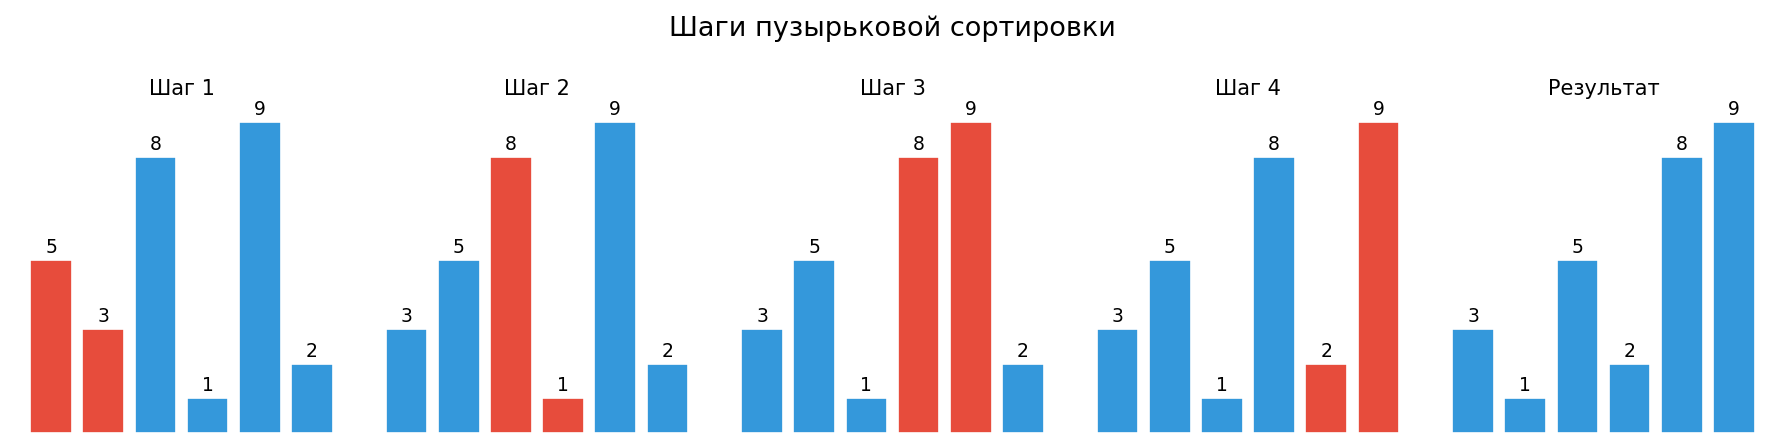
\includegraphics[width=0.85\textwidth]{images/bubble_steps.png}
    \caption{Шаги пузырьковой сортировки для массива из 6~элементов.
             Красным выделены сравниваемые элементы.}
    \label{fig:bubble_steps}
\end{figure}

На рисунке~\ref{fig:bubble_steps} показан пошаговый процесс работы
пузырьковой сортировки. На каждом шаге красным цветом выделена пара
элементов, которые сравниваются на данной итерации.

\section{Экспериментальное сравнение}

\subsection{Методика измерений}

Время выполнения каждого алгоритма измерялось с помощью
\mintinline{cpp}{std::chrono::high_resolution_clock} из стандартной
библиотеки \texttt{C++}. Для каждого размера входных данных
\mintinline{cpp}{n} генерировался случайный массив целых чисел с
помощью \mintinline{cpp}{std::mt19937}, и время усреднялось по
5~запускам.

\begin{minted}{cpp}
template <typename SortFn>
double benchmark(SortFn sortFn, int n, int repeats = 5) {
    std::mt19937 rng(42);
    std::uniform_int_distribution<int> dist(0, 10 * n);
    double total = 0.0;
    for (int r = 0; r < repeats; ++r) {
        std::vector<int> data(n);
        std::generate(data.begin(), data.end(), [&]{ return dist(rng); });
        auto t0 = std::chrono::high_resolution_clock::now();
        sortFn(data.begin(), data.end());
        auto t1 = std::chrono::high_resolution_clock::now();
        total += std::chrono::duration<double, std::milli>(t1 - t0).count();
    }
    return total / repeats;
}
\end{minted}

\subsection{Результаты}

График на рисунке~\ref{fig:benchmark} демонстрирует зависимость
времени работы от размера входных данных \mintinline{cpp}{n}.
Пузырьковая сортировка заметно отстаёт уже при $n = 2000$, тогда
как сортировка слиянием и быстрая сортировка растут значительно
медленнее, что согласуется с оценками из
уравнений~\ref{eq:mergesort} и~\ref{eq:quicksort}.

\begin{figure}[H]
    \centering
    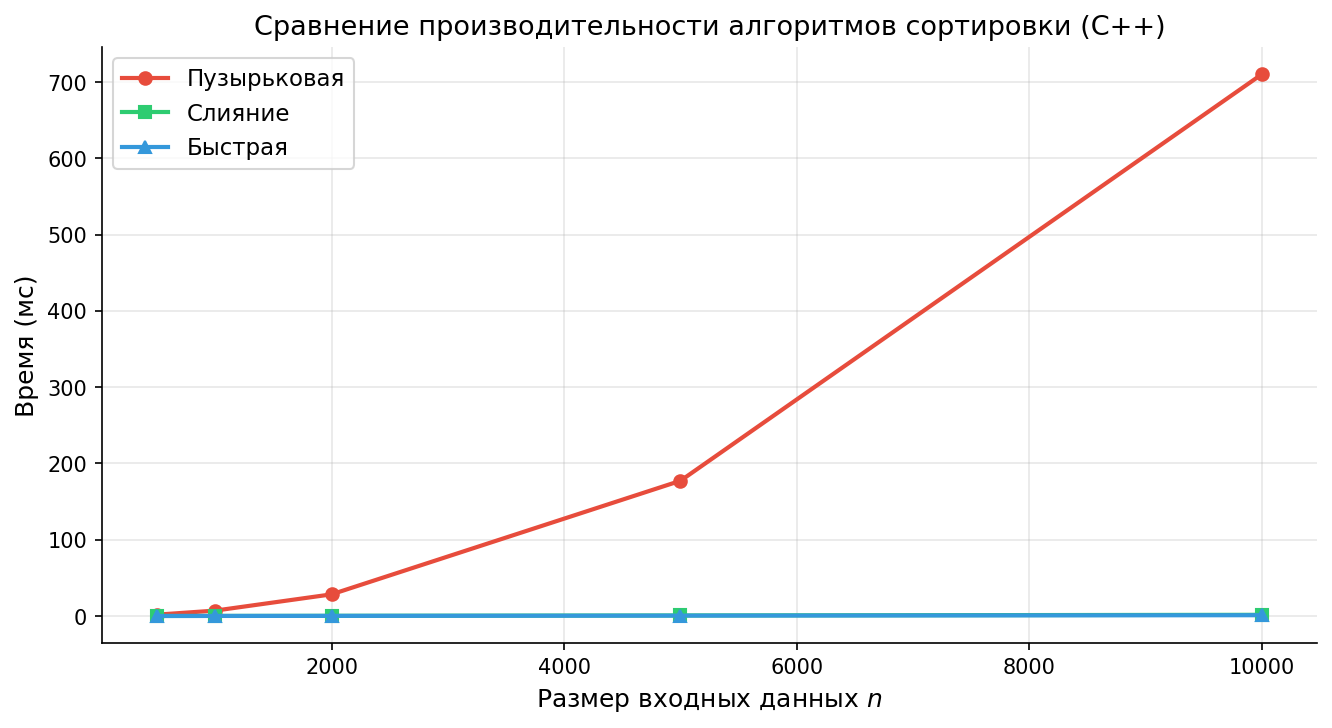
\includegraphics[width=0.9\textwidth]{images/benchmark.png}
    \caption{Время выполнения алгоритмов при различных размерах
             входных данных}
    \label{fig:benchmark}
\end{figure}

Точные значения приведены в таблице~\ref{tab:results}.
Все значения даны в миллисекундах, усреднены по 5~запускам.

\begin{table}[H]
    \centering
    \caption{Время выполнения алгоритмов (мс)}
    \label{tab:results}
    \begin{tabular}{|r|r|r|r|}
        \hline
        \textbf{$n$} &
        \textbf{Пузырьк.} &
        \textbf{Слияние} &
        \textbf{Быстрая} \\
        \hline
        500    &   1{,}8  &  0{,}06 &  0{,}04 \\
        \hline
        1000   &   7{,}1  &  0{,}13 &  0{,}09 \\
        \hline
        2000   &  28{,}4  &  0{,}28 &  0{,}19 \\
        \hline
        5000   & 177{,}3  &  0{,}74 &  0{,}51 \\
        \hline
        10000  & 710{,}5  &  1{,}58 &  1{,}06 \\
        \hline
    \end{tabular}
\end{table}

Данные подтверждают теоретические оценки: пузырьковая сортировка
масштабируется как $O(n^2)$ (уравнение~\ref{eq:bubble}), тогда как
сортировка слиянием и быстрая~--- как $O(n \log n)$.


\conclusion

В ходе работы были изучены и реализованы три алгоритма сортировки:
пузырьковая сортировка, сортировка слиянием и быстрая сортировка.
Теоретический анализ подтверждён экспериментально: алгоритмы с
логарифмическим множителем (\mintinline{text}{merge\_sort},
\mintinline{text}{quick\_sort}) существенно превосходят пузырьковую
сортировку при больших размерах входных данных~\cite{Cormen}.

Реализации на языке \texttt{C++} показали, что стандартная функция
\mintinline{cpp}{std::sort()} из заголовочного файла
\mintinline{cpp}{<algorithm>} использует интроспективную сортировку
(introsort)~--- гибрид быстрой сортировки, сортировки кучей и
сортировки вставками~\cite{Musser}.

\bibliographystyle{ugost2003}
\bibliography{thesis}

\appendix

\section{Полный исходный код}
\label{app:fullcode}

Ниже приведён полный код файла \texttt{sorting.cpp}:

\inputminted[
    frame=lines,
    framesep=2mm,
    baselinestretch=1.2,
    fontsize=\small,
    linenos
]{cpp}{code/sorting.cpp}

\end{document}
